\section{超越无损推测：操作系统超参数调优环境}
\label{sec:os-speculation}

到目前为止，我们的实验都聚焦于\emph{无损}推测：推测动作必须逐步验证之后才能提交。现在我们转向一个放宽这一逐步约束的\emph{有损}场景。
在操作系统这类对延迟极其敏感的环境中，等待一个强大但缓慢的 Actor（需要 10--15 秒进行思考）可能会让系统长时间停留在退化状态。
我们的框架使用一个快速的 Speculator 立即施加调整，
在 Actor 还在思考时就改善实时性能。
其安全性由“最后写入者获胜”（last-write-wins）机制保证——Actor 的最终决策会直接覆盖任何推测动作，
从而无需复杂回滚。
这种方法加快了收敛，并提升了响应速度；
我们在 \texttt{sysbench cpu} 基准上评估这一点，该基准是一个 CPU 密集型工作负载\citep{sysbench}。

\subsection{实验设置}

我们调节 Linux 完全公平调度器（CFS）的一个参数 \texttt{min\_granularity}，
它控制任务的最小时片长度。
这个参数会强烈影响调度性能：较小的时片可以降低延迟，但可能损害吞吐；这是一个经典权衡。已有工作\citep{liargkovas2025llmTuning} 证明，基于 LLM 的智能体可以优化这一参数；在此基础上，我们进一步引入了推测式控制回路。

我们的系统由一个快速的 Speculator 和一个缓慢的 Actor 构成。
Speculator 每秒根据最新性能指标提出一次有界的参数更新。
相比之下，Actor 每 10--15 秒响应一次；它会分析近期由 Speculator 产生的压缩版（测量值，动作）序列。
当 Actor 的响应到达时，其选定设置会被立刻应用，并用来更新 Speculator 的上下文，
从而保证后续快速步骤建立在经过验证的叙述之上，而不是不断漂移。

\vspace{-3pt}
\paragraph{评估}
我们评估三种系统：
\begin{enumerate}[leftmargin=*]
    \item \textbf{仅 Actor}：较慢，但更具审慎分析能力（10--15\,秒一个决策周期）；
    \item \textbf{仅 Speculator}：较快（1\,秒一个决策周期），但分析不够深入；
    \item \textbf{Speculator--Actor}：在 Actor 决策之间插入推测更新的联合系统。
\end{enumerate}
我们关心三个方面：(i) 响应时间，(ii) 收敛到最优设置的速度，以及 (iii) 是否能够避免“仅 Speculator”基线容易陷入的局部最优。

\vspace{-5pt}
\subsection{结果}
\begin{figure*}[t]
 \centering
 \begin{minipage}[c]{0.64\linewidth}
  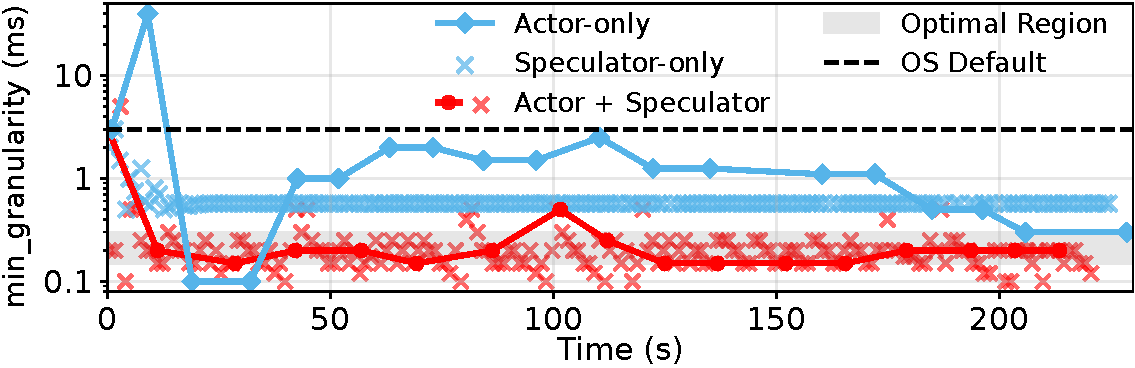
\includegraphics[width=\linewidth]{figures/os_tuning/combined_plot.pdf}
 \end{minipage}
 \hfill
 \begin{minipage}[c]{0.35\linewidth}
  \centering
\begin{tabular}{l p{1.5cm}}
  \toprule
  \textbf{配置} & \textbf{p95 延迟 (ms)} \\
  \midrule
  未调优 & 102.97\\
  仅 Actor & 54.00 \\
  Actor + Spec. & 37.93 \\
  \bottomrule
\end{tabular}
 \end{minipage}
 \caption{
 \textbf{（左）} \textbf{Speculator--Actor}、\textbf{仅 Speculator} 与 \textbf{仅 Actor} 的收敛过程对比。
 Speculator 缩短了系统在糟糕设置上的探索时间。
 \textbf{仅 Speculator} 虽然稳定得很快，但最终值更差。
 \textbf{（右）} 一个 20 秒调优实验中的平均 p95 延迟，说明快速反应能立刻带来性能收益（见 \S\ref{app:speculative-mitigation}）。数值越低越好。}
 \label{fig:os-speculation}
\end{figure*}
\vspace{-8pt}

\paragraph{Speculator 缓解了慢响应带来的性能恶化}
正如\cref{fig:os-speculation}（右）所示，Speculator 显著改善了系统的反应速度。在恢复阶段，完整的 Speculator--Actor 系统将平均 p95 延迟维持在 37.93 ms。这相较于仅 Actor 的基线有明显提升：后者不得不在较差配置下停留更久，平均延迟达到 54.00 ms。Speculator 的快速纠偏避免了系统长期停留在高延迟状态（初始值为 102.97 ms），因此即便 Actor 仍在较慢地思考，也能立刻带来收益（完整实验细节见 \S\ref{app:speculative-mitigation}）。

\paragraph{Speculator 加速收敛到最优值}
Speculator 的高频更新也显著加快了收敛。
如\cref{fig:os-speculation}（左）所示，Speculator--Actor 系统大约在 10--15 秒内就能到达一个最优设置（例如 \texttt{min\_granularity} = 0.2\,ms）。
相比之下，仅 Actor 智能体大约需要 200 秒——慢了约 20 倍——并且在很长一段时间内都被困在高度次优的状态中（例如延迟 $>$120\,ms）。
Speculator 的快速探索为 Actor 提供了更丰富的性能地形信息，使其能够更快地把系统从这些病态区域中拉出来。

\paragraph{仅 Speculator 很快，但并不最优}
\cref{fig:os-speculation} 还显示，尽管仅 Speculator 系统响应很快，但它会过早收敛到一个次优配置：\texttt{min\_granularity} 为 0.55\,ms（36.24\,ms 延迟）。
这一结果明显劣于完整 Speculator--Actor 系统达到的 0.2\,ms（30.26\,ms 延迟）。没有 Actor 的指导，Speculator 缺乏足够的推理深度，无法跳出这一局部最优。

联合的 Speculator--Actor 系统将快速适应与策略性指导结合起来，同时实现了高响应性与最优稳态性能。
